% !TEX root = ../main.tex

\section{Proposal}
\label{sec:proposal}
As discussed in section~\ref{sect:vul}, three major vulnerabilities are in the scope of this project. We summarized each security vulnerability and the corresponding mitigation plan in table~\ref{tbl:attack}. There are references to line numbers in our secure ERC20 implementation. Required comments have been added to the code to clarify usage of each section.
\begin{table}[t]
	\begin{tabular}{|l|l|l|l|}
		\hline
		\textbf{} & \textbf{Vulnerability}     & \textbf{Mitigation}                            & \textbf{Line\#} \\ \hline		\hline
		1           & Overflow attack            & Using SafeMath library                         & 30-131                \\ \hline
		2           & Multiple Withdrawal attack & Securing \texttt{transferFrom} method                   & 218-221              \\ \hline
		3           & Re-entrancy attack         & Preventing the attack in the \texttt{fallback} \& \texttt{sell} functions & 161, 262 \& 279              \\ \hline
	\end{tabular}
	\caption{Major ERC20 vulnerabilities with their corresponding mitigation plan. The last column refers to the respective line number in the implemented code.}
	\label{tbl:attack}
\end{table}

By using \texttt{SafeMath} library each arithmetic operation needs to be replaced by its \texttt{SafeMath} equivalent. For example, $a+b$ will be replaced by $a.add(b)$. This prevent integer overflow and mitigate the attack. Adding recommended code by \cite{ERC20MWA} in the \texttt{transferFrom} method keeps track of transferred tokens and prevent multiple withdrawal attack. Finally, \texttt{fallback} function logs an event to track transferred Ether to the contract. This is inline with minimum recommended Gas to prevent re-entrancy attack. In general, the code can be divided into the following sections:
\begin{enumerate}[]
	\item \textbf{Lines 1-27:} Declaring ERC20 interface as guideline of requires functions
	\item \textbf{Lines 30-131:} Declaring \texttt{SafeMath} library to be used in the main code. Using this library mitigates~\ref{sect:overflow} attack (Integer overflow attack).
	\item \textbf{Lines 139-324:} Implementing ERC20 functions by considering security measurements. Line 218-221 mitigates~\ref{sect:withdrawal} (Multiple withdrawal attack) and using locking approach in line 161, 262 and 279 mitigates~\ref{sect:reentrancy} (Re-entrancy attack).
\end{enumerate}

We implemented and tested our ERC20 proposal\footnote{\url{https://rinkeby.etherscan.io/address/0xd337819ec1530c69ae9323364d4865d5659057ca\#code}} on Rinkeby test network. It can be similarly implemented on private blockchain since MetaMask supports it\footnote{Connecting MyEtherWallet, Mist, and MetaMask to Your Private Blockchain \url{https://bitfalls.com/2018/03/26/connecting-myetherwallet-mist-metamask-private-blockchain/}}. We initially tested our code on a private blockchain based on Ganache\footnote{A private Ethereum blockchain to run tests. It gives the ability to perform all actions similar to the main chain without the cost \url{https://www.trufflesuite.com/docs/ganache/quickstart}.}
\par

%\begin{lstlisting}[basicstyle=\scriptsize\ttfamily,caption={Secure ERC20 proposal addressing three major security vulnerabilities.},label={code:prop}]
%pragma solidity ^0.5.2;
%
%/** 
%* For new ERC20 token deployments:
%* 1- Install MetaMask Chrome/Firefox extension.
%* 2- Connect MetaMask to Rinkeby Testnet (or your private chain).
%* 3- Run RemixIDE and set environment="Injected Web3".
%* 4- Copy and past this code to RemixIDE.
%* 5- Deploy the token (EST contract) on the blockchain.
%* 6- Use MetaMask for importing the token and interacting with it.
%*/
%
%/**
%* ERC20 interface
%* https://theethereum.wiki/w/index.php/ERC20_Token_Standard
%*/
%contract ERC20 {
%function totalSupply() external view returns (uint256);
%function balanceOf(address _account) external view returns (uint256);
%function transfer(address _to, uint256 _tokens) external returns (bool);
%function approve(address _spender, uint256 _tokens) external returns (bool);
%function transferFrom(address _from, address _to, uint256 _tokens) external returns (bool);
%function allowance(address _account, address _spender) external view returns (uint256);
%
%event Transfer(address indexed _from, address indexed _to, uint256 _tokens);
%event Approval(address indexed _tokenOwner, address indexed _spender, uint256 _tokens);
%}
%
%
%/**
%* https://github.com/OpenZeppelin/openzeppelin-contracts/blob/master/contracts/math/SafeMath.sol
%* @dev Wrappers over Solidity's arithmetic operations with added overflow checks.
%*
%* Arithmetic operations in Solidity wrap on overflow. This can easily result
%* in bugs, because programmers usually assume that an overflow raises an
%* error, which is the standard behavior in high level programming languages.
%* `SafeMath` restores this intuition by reverting the transaction when an
%* operation overflows.Using this library instead of the unchecked operations
%* eliminates an entire class of bugs, so it's recommended to use it always.
%*/
%library SafeMath {
%/**
%* @dev Returns the addition of two unsigned integers, reverting on overflow.
%*
%* Counterpart to Solidity's `+` operator.
%*
%* Requirements:
%* - Addition cannot overflow.
%*/
%function add(uint256 a, uint256 b) internal pure returns (uint256) {
%uint256 c = a + b;
%require(c >= a, "SafeMath: addition overflow");
%
%return c;
%}
%
%/**
%* @dev Returns the subtraction of two unsigned integers, reverting on
%* overflow (when the result is negative).
%*
%* Counterpart to Solidity's `-` operator.
%*
%* Requirements:
%* - Subtraction cannot overflow.
%*/
%function sub(uint256 a, uint256 b) internal pure returns (uint256) {
%require(b <= a, "SafeMath: subtraction overflow");
%uint256 c = a - b;
%
%return c;
%}
%
%/**
%* @dev Returns the multiplication of two unsigned integers, reverting on
%* overflow.
%*
%* Counterpart to Solidity's `*` operator.
%*
%* Requirements:
%* - Multiplication cannot overflow.
%*/
%function mul(uint256 a, uint256 b) internal pure returns (uint256) {
%// Gas optimization: this is cheaper than requiring 'a' not being zero, but the
%// benefit is lost if 'b' is also tested.
%// See: https://github.com/OpenZeppelin/openzeppelin-solidity/pull/522
%if (a == 0) {
%return 0;
%}
%
%uint256 c = a * b;
%require(c / a == b, "SafeMath: multiplication overflow");
%
%return c;
%}
%
%/**
%* @dev Returns the integer division of two unsigned integers. Reverts on
%* division by zero. The result is rounded towards zero.
%*
%* Counterpart to Solidity's `/` operator. Note: this function uses a
%* `revert` opcode (which leaves remaining gas untouched) while Solidity
%* uses an invalid opcode to revert (consuming all remaining gas).
%*
%* Requirements:
%* - The divisor cannot be zero.
%*/
%function div(uint256 a, uint256 b) internal pure returns (uint256) {
%// Solidity only automatically asserts when dividing by 0
%require(b > 0, "SafeMath: division by zero");
%uint256 c = a / b;
%// assert(a == b * c + a % b); // There is no case in which this doesn't hold
%
%return c;
%}
%
%/**
%* @dev Returns the remainder of dividing two unsigned integers. (unsigned integer modulo),
%* Reverts when dividing by zero.
%*
%* Counterpart to Solidity's `%` operator. This function uses a `revert`
%* opcode (which leaves remaining gas untouched) while Solidity uses an
%* invalid opcode to revert (consuming all remaining gas).
%*
%* Requirements:
%* - The divisor cannot be zero.
%*/
%function mod(uint256 a, uint256 b) internal pure returns (uint256) {
%require(b != 0, "SafeMath: modulo by zero");
%return a % b;
%}
%}
%
%/**
%*  Concordia University
%*  Montreal, Canada
%*  INSE6610 project : Summer 2019
%*  On Secure Ethereum Token
%*/
%contract EST is ERC20{
%using SafeMath for uint256;		// Using SafeMath to mitigate integer overflow
%
%string public constant name = "Ethereum Secure Token";  // Name of the token
%string public constant symbol = "EST";                  // Token symbol
%
%uint8 public exchangeRate = 100;        // 1 ETH = 100 tokens
%uint256 private decimals = 10 ** 18;    // Divisible to 18 decimal places
%
%mapping(address => mapping (address => uint256)) private allowed;		// Allowed token to transfer by spender
%mapping(address => mapping (address => uint256)) private transferred;	// Transferred tokens by spender
%mapping(address => uint256) balances;                                   // Balance of token holders
%
%address payable private owner = address(0);     // Owner of the token
%uint256 private _totalSupply = 100000000;       // Control economy of the token
%
%// Log events when buying/selling tokens or sending/withdrawing ETH
%event LogBuy(address indexed _buyer, uint256 _wei, address indexed _owner, uint256 _tokens);
%event LogSell(address indexed _seller, uint256 _tokens, address indexed _contract, uint256 _wei, address indexed _owner);
%event LogReceived(address indexed _sender, uint256 _wei);
%event LogWithdrawal(address indexed _from, address _contract, uint256 _wei, address indexed _to);
%
%bool private locked = false;                    // Lock variable to mitigate re-entrancy attack
%
%/**
%* Accepts Ether and logs an event
%*/ 
%function() external payable{
%emit LogReceived(msg.sender, msg.value);    // Logs sender of ETH (2300 max gas)
%}
%
%/**
%* Token constructor
%*/
%constructor() public {
%owner = msg.sender;                             // Owner of the contract
%balances[owner] = _totalSupply;                 // Assigning initial tokens to the owner
%emit Transfer(address(0), owner, _totalSupply); // Logs transfered tokens to the owner
%}
%
%/**
%* Returns total amount of token in circulation
%*/
%function totalSupply() public view returns (uint256 tokens) {
%return _totalSupply;    // Total supply of the token
%}
%
%/**
%* Get the token balance for an address
%*/
%function balanceOf(address _tokenHolder) public view returns (uint256 tokens) {
%return balances[_tokenHolder];                              // Balance of token holder
%}
%
%/**
%* Transfer the balance (value) from owner's account to another account
%*/
%function transfer(address _to, uint256 _tokens) public returns (bool success) {
%require(_tokens > 0);                                       // Check for more than zero token
%require(balances[msg.sender] >= _tokens);                   // Check if the sender has enough
%require(balances[_to] + _tokens >= balances[_to]);          // Check for overflows
%balances[msg.sender] = balances[msg.sender].sub(_tokens);   // Subtract from the sender
%balances[_to] = balances[_to].add(_tokens);                 // Add the same to the recipient
%emit Transfer(msg.sender, _to, _tokens);
%return true;
%}
%
%/**
%* Special type of Transfer and make it possible to give permission to another address 
%* to spend token on your behalf.
%* It sends _tokens amount of tokens from address _from to address _to
%* The transferFrom method is used for a withdraw work-flow, allowing contracts to send
%* tokens on your behalf, for example to "deposit" to a contract address and/or to charge
%* fees in sub-currencies; the command should fail unless the _from account has
%* deliberately authorized the sender of the message via some mechanism
%*/
%function transferFrom(address _from, address _to, uint256 _tokens) public returns (bool success) {
%require(_to != address(0));                         // Receiver is valid?
%require(balances[_from] >= _tokens);                // Checks if approver has enough tokens
%require(_tokens <= (                                // Mitigates multiple Withdrawal Attack
%(allowed[_from][msg.sender] > transferred[_from][msg.sender]) ? 
%allowed[_from][msg.sender].sub(transferred[_from][msg.sender]) : 0)
%);                              // Prevent token transfer more than allowance
%
%balances[_from] = balances[_from].sub(_tokens);     // Decrease balance of approver
%transferred[_from][msg.sender] = transferred[_from][msg.sender].add(_tokens);   // Tracks transferred tokens
%balances[_to] = balances[_to].add(_tokens);         // Increases balance of spender
%emit Transfer(_from, _to, _tokens);                 // Logs transferred tokens
%return true;
%}
%
%/**
%* It helps to give permission to another address to spend tokens on your behalf.
%* Allow _spender to withdraw from your account, multiple times, up to the _tokens amount.
%* If this function is called again it overwrites the current allowance with _tokens.
%*/
%function approve(address _spender, uint256 _tokens) public returns (bool success) {
%require(_spender != address(0));                // Is address valid?
%require(_spender != msg.sender);                // Spender cannot approve himself
%require(balances[msg.sender] >= _tokens);       // Approve has enough tokens?
%allowed[msg.sender][_spender] = _tokens;        // Sets allowance of the spender
%emit Approval(msg.sender, _spender, _tokens);   // Logs approved tokens
%return true;
%}
%
%/**
%* Returns the amount of tokens approved by the owner that can be
%* transferred to the spender's account. In other word, how many tokens we gave
%* permission to another address to spend
%*/
%function allowance(address _tokenHolder, address _spender) public view returns (uint256 tokens) {
%return allowed[_tokenHolder][_spender];     // returns allowance of _spender
%}
%
%/**
%* Transferring ETH to the seller of the token
%* If it was not successful, it will revert everything
%*/
%function sell(uint256 _tokens) public returns(bool success)
%{
%require(_tokens > 0);                       // Is there any token to sell?
%require(balances[msg.sender] >= _tokens);   // Seller has enough tokens?
%require(!locked);                           // Lock=false -> no recursive call -> safe to proceed
%locked = true;                              // Sets lock=true to mitigate re-entrancy attack
%
%uint256 _wei = _tokens.div(exchangeRate).mul(decimals);     // Token to ETH and then ETH to Wei
%if (address(this).balance >= _wei)                          // Contract has enough Wei to send?
%{
%msg.sender.transfer(_wei);                                  // Transferring Wei
%balances[msg.sender] = balances[msg.sender].sub(_tokens);   // Decreasing tokens of seller
%balances[owner] = balances[owner].add(_tokens);             // Increasing tokens of owner
%emit LogSell(msg.sender, _tokens, address(this), _wei, owner);
%success = true;                         // Seller sold _tokens to owner and Contract paid _wei
%}
%else
%{
%emit LogSell(msg.sender, 0, address(this), 0, owner);  // Logs failed transfer (zero)
%success = false;
%}
%
%locked = false;     // Unlocks the function
%return success;
%}
%
%/**
%* Transferring ETH to the address that is specified by the owner
%* Only owner of the contract can call this function
%*/
%function send(address payable _to, uint256 _eth) public onlyOwner returns(bool success){
%uint256 _wei = _eth.mul(decimals);          // ETH to Wei
%require(address(this).balance >= _wei);     // Contract has enough ETH?
%_to.transfer(_wei);                         // Transferring Wei to _to
%emit LogWithdrawal(owner, address(this), _wei, _to);  
%return true;                // Owner requested the Contract to send _wei to _to
%}
%
%/**
%* Buying token by transferring ETH
%*/
%function buy() public payable returns(bool success){
%require(msg.sender != owner);               // Token owner cannot be as seller and buyer
%uint256 _eth = msg.value.div(decimals);     // Wei to ETH
%uint256 _tokens = _eth.mul(exchangeRate);   // ETH to Token
%require(balances[owner] >= _tokens);        // Owner has enough tokens?
%
%balances[msg.sender] = balances[msg.sender].add(_tokens);   // Increasing token balance of buyer
%balances[owner] = balances[owner].sub(_tokens);             // Decreasing token balance of owner
%emit LogBuy(msg.sender, msg.value, owner, _tokens);         // Buyer sent _wei and Owner sold _tokens
%return true;
%}
%
%/**
%* Returns ETH balance of the Contract to the contract owner
%*/
%function contractBalance() public view onlyOwner returns(uint256 eth){
%return address(this).balance.div(decimals); // Wei to ETH
%}
%
%/**
%* Checks if the caller is contract owner
%*/
%modifier onlyOwner() {
%require(msg.sender == owner);
%_;
%}
%}
%\end{lstlisting}

In terms of compatibly, we used MetaMask\footnote{An extension for accessing Ethereum enabled distributed applications in the browser. The extension injects the Ethereum web3 API into every website's javascript context, so that DApps can read from the blockchain.\url{https://metamask.io/}} to test our deployed token. MetaMask did not raise any transfer issue which shows compatibility of the token with existing wallets (see figure~\ref{fig:propwallet}).

\begin{figure}[t]
	\centering
	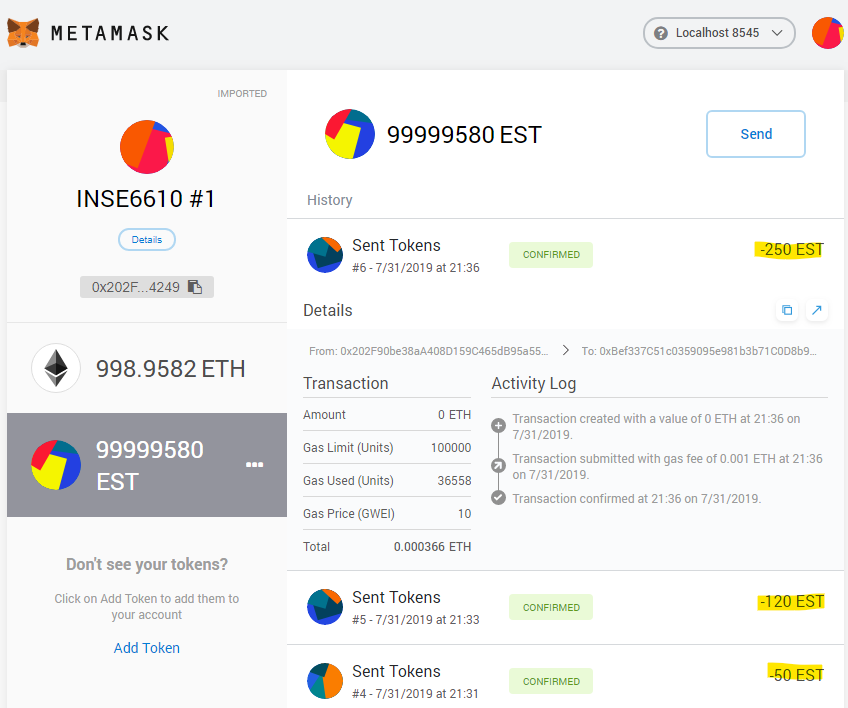
\includegraphics[width=0.9\linewidth]{figures/img19.png}
	\caption{Compatibility of deployed token with existing wallets (MetaMask)}
	\label{fig:propwallet}
\end{figure}

Moreover, transferring and receiving tokens trigger expected events (see figure~\ref{fig:proptran})

\begin{figure}[t]
	\centering
	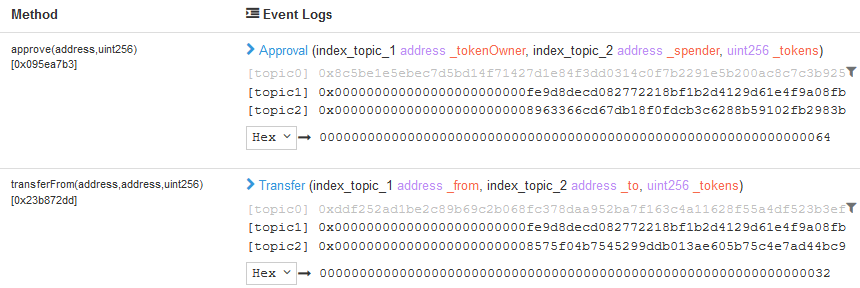
\includegraphics[width=1.0\linewidth]{figures/img18.png}
	\caption{Logged events by the token contract after calling \texttt{Approve} or \texttt{transferFrom}}
	\label{fig:proptran}
\end{figure}

In addition to standard ERC20 methods, this implementation extends ERC20 functionalities by introducing new features:

\begin{enumerate}
	\item \textbf{Selling tokens:} Token holders can send back tokens to the contract and receive ETH in return. They will receive ETH based on current exchange rate of the contract (managed by \texttt{exchangeRate} variable). Currently, this exchange rate is 100 tokens for 1 ETH. For example, if someone sends 200 tokens to the contract, the contract will send him/her back 2 ETH. This functionality is implemented by \texttt{sell(uint256 \_tokens)} function and accepts a payable address for returning ETH to it. After each exchange, the function logs \texttt{LogSell} event which helps to track exchanged tokens for ETH.
	\item \textbf{Buying tokens:} Users can call \texttt{buy()} function to purchase autonomously tokens. This function is defined as \textit{payable}\footnote{Payable functions provide a mechanism to collect/receive funds in ethers. Payable functions are annotated with payable keyword.} and accept ETH. It then calculates number of token based on current exchange rate and increases balance of the caller. Like \texttt{sell} function, it logs \texttt{LogBuy} event for tracking purchased tokens.
	\item \textbf{Withdrawing ETH:} This function can be called only by the owner of the contract. Since contract accepts ETH, token owner may use this function to transfer ETH out of the contract. Otherwise, received ETH by the contract will stick in the contract and would not be usable. There is a complementary function (i.e., \texttt{contractBalance()}) to get current ETH balance of the contract. This function also can be called by the owner to see how many ETH are under the contract. Transferring ETH out of the contract also logs \texttt{LogWithdrawal} event which logs moved ETH from the contract.
\end{enumerate}

\begin{figure}[t]
	\centering
	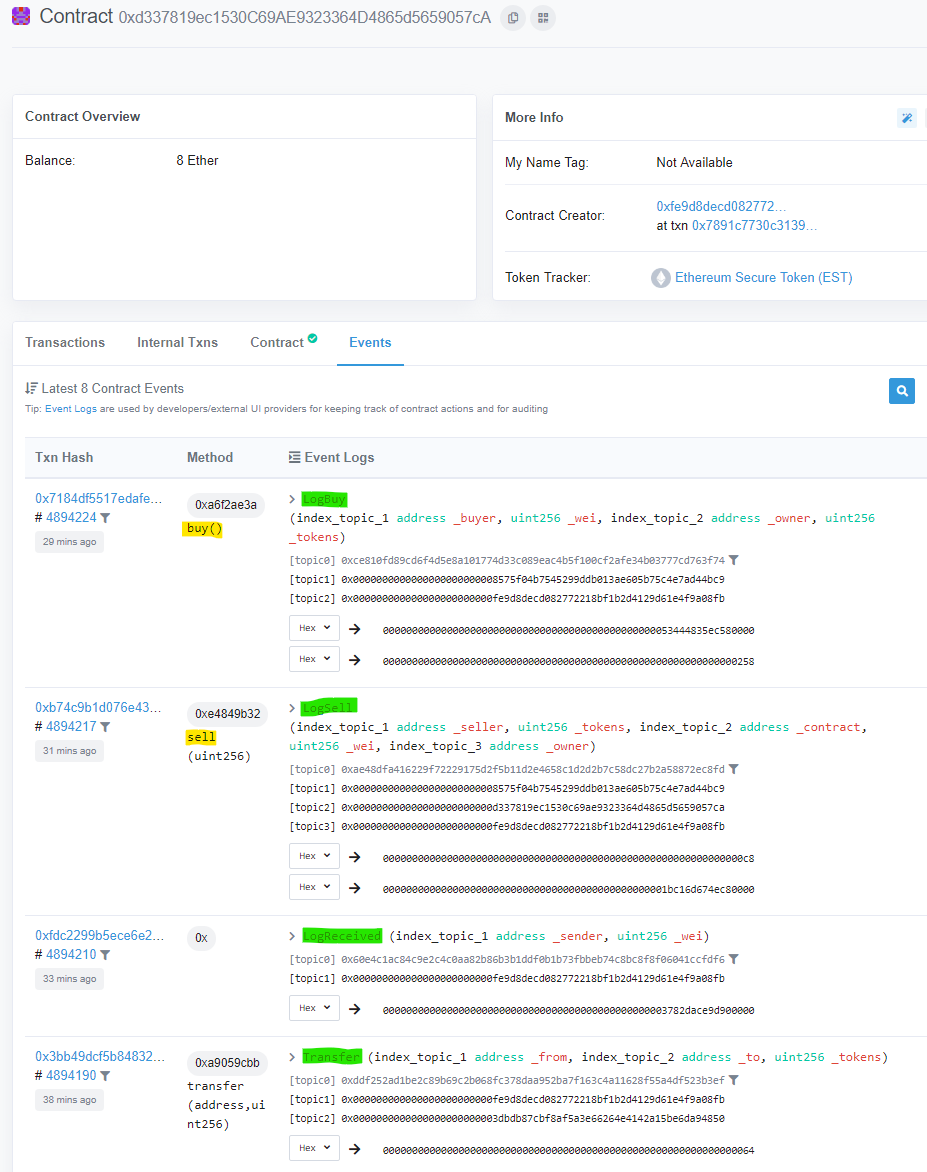
\includegraphics[width=1.0\linewidth]{figures/img20.png}
	\caption{Added functionalities to the ERC20 contract. Each new feature logs corresponding event to track transactions of the token.}
	\label{fig:propevents}
\end{figure}